	\begin{frame}
	\frametitle{День 1. 18 августа}
	\framesubtitle{Старт~--- д.р. Кичкинакол Уллукёльский} % Optional subtitle
	\begin{columns}[c] % The "c" option specifies centered vertical alignment while the "t" option is used for top vertical alignment
		\begin{column}{0.45\textwidth} % Left column width
			\begin{itemize}
				\item Перепаковка, формирование заброски
				\item Прошли \textbf{5.3} км
				\item ЧХВ: 2:46
				\item Набор/сброс: \textcolor{darkred}{\textbf{+650}}/\textcolor{darkblue}{\textbf{-0}}~м
			\end{itemize}
			
		\end{column}
		\begin{column}{0.5\textwidth} % Right column width
			\centering
			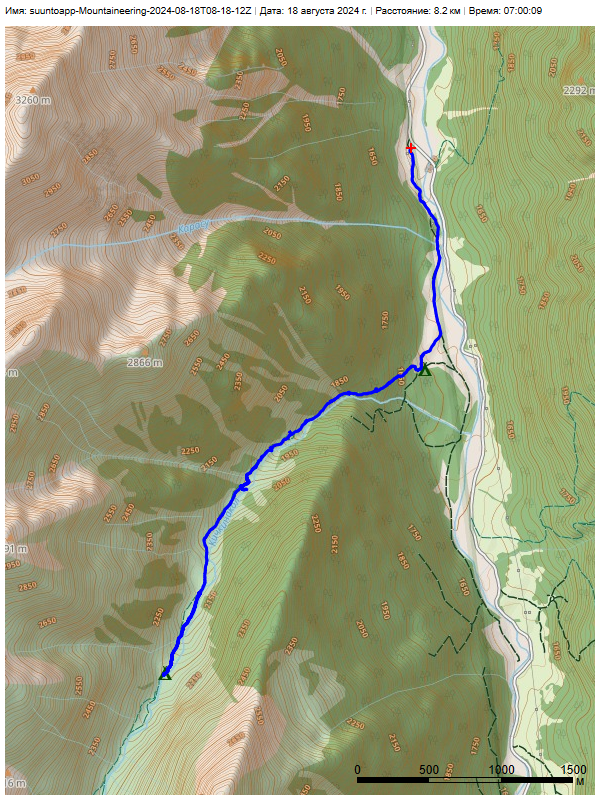
\includegraphics[width=\linewidth]{../pics/mini_maps/18}
		\end{column}
	\end{columns}
\end{frame}

\begin{frame}
	\frametitle{Выход на маршрут}
	\framesubtitle{День 1, 18 августа}
	\centering
	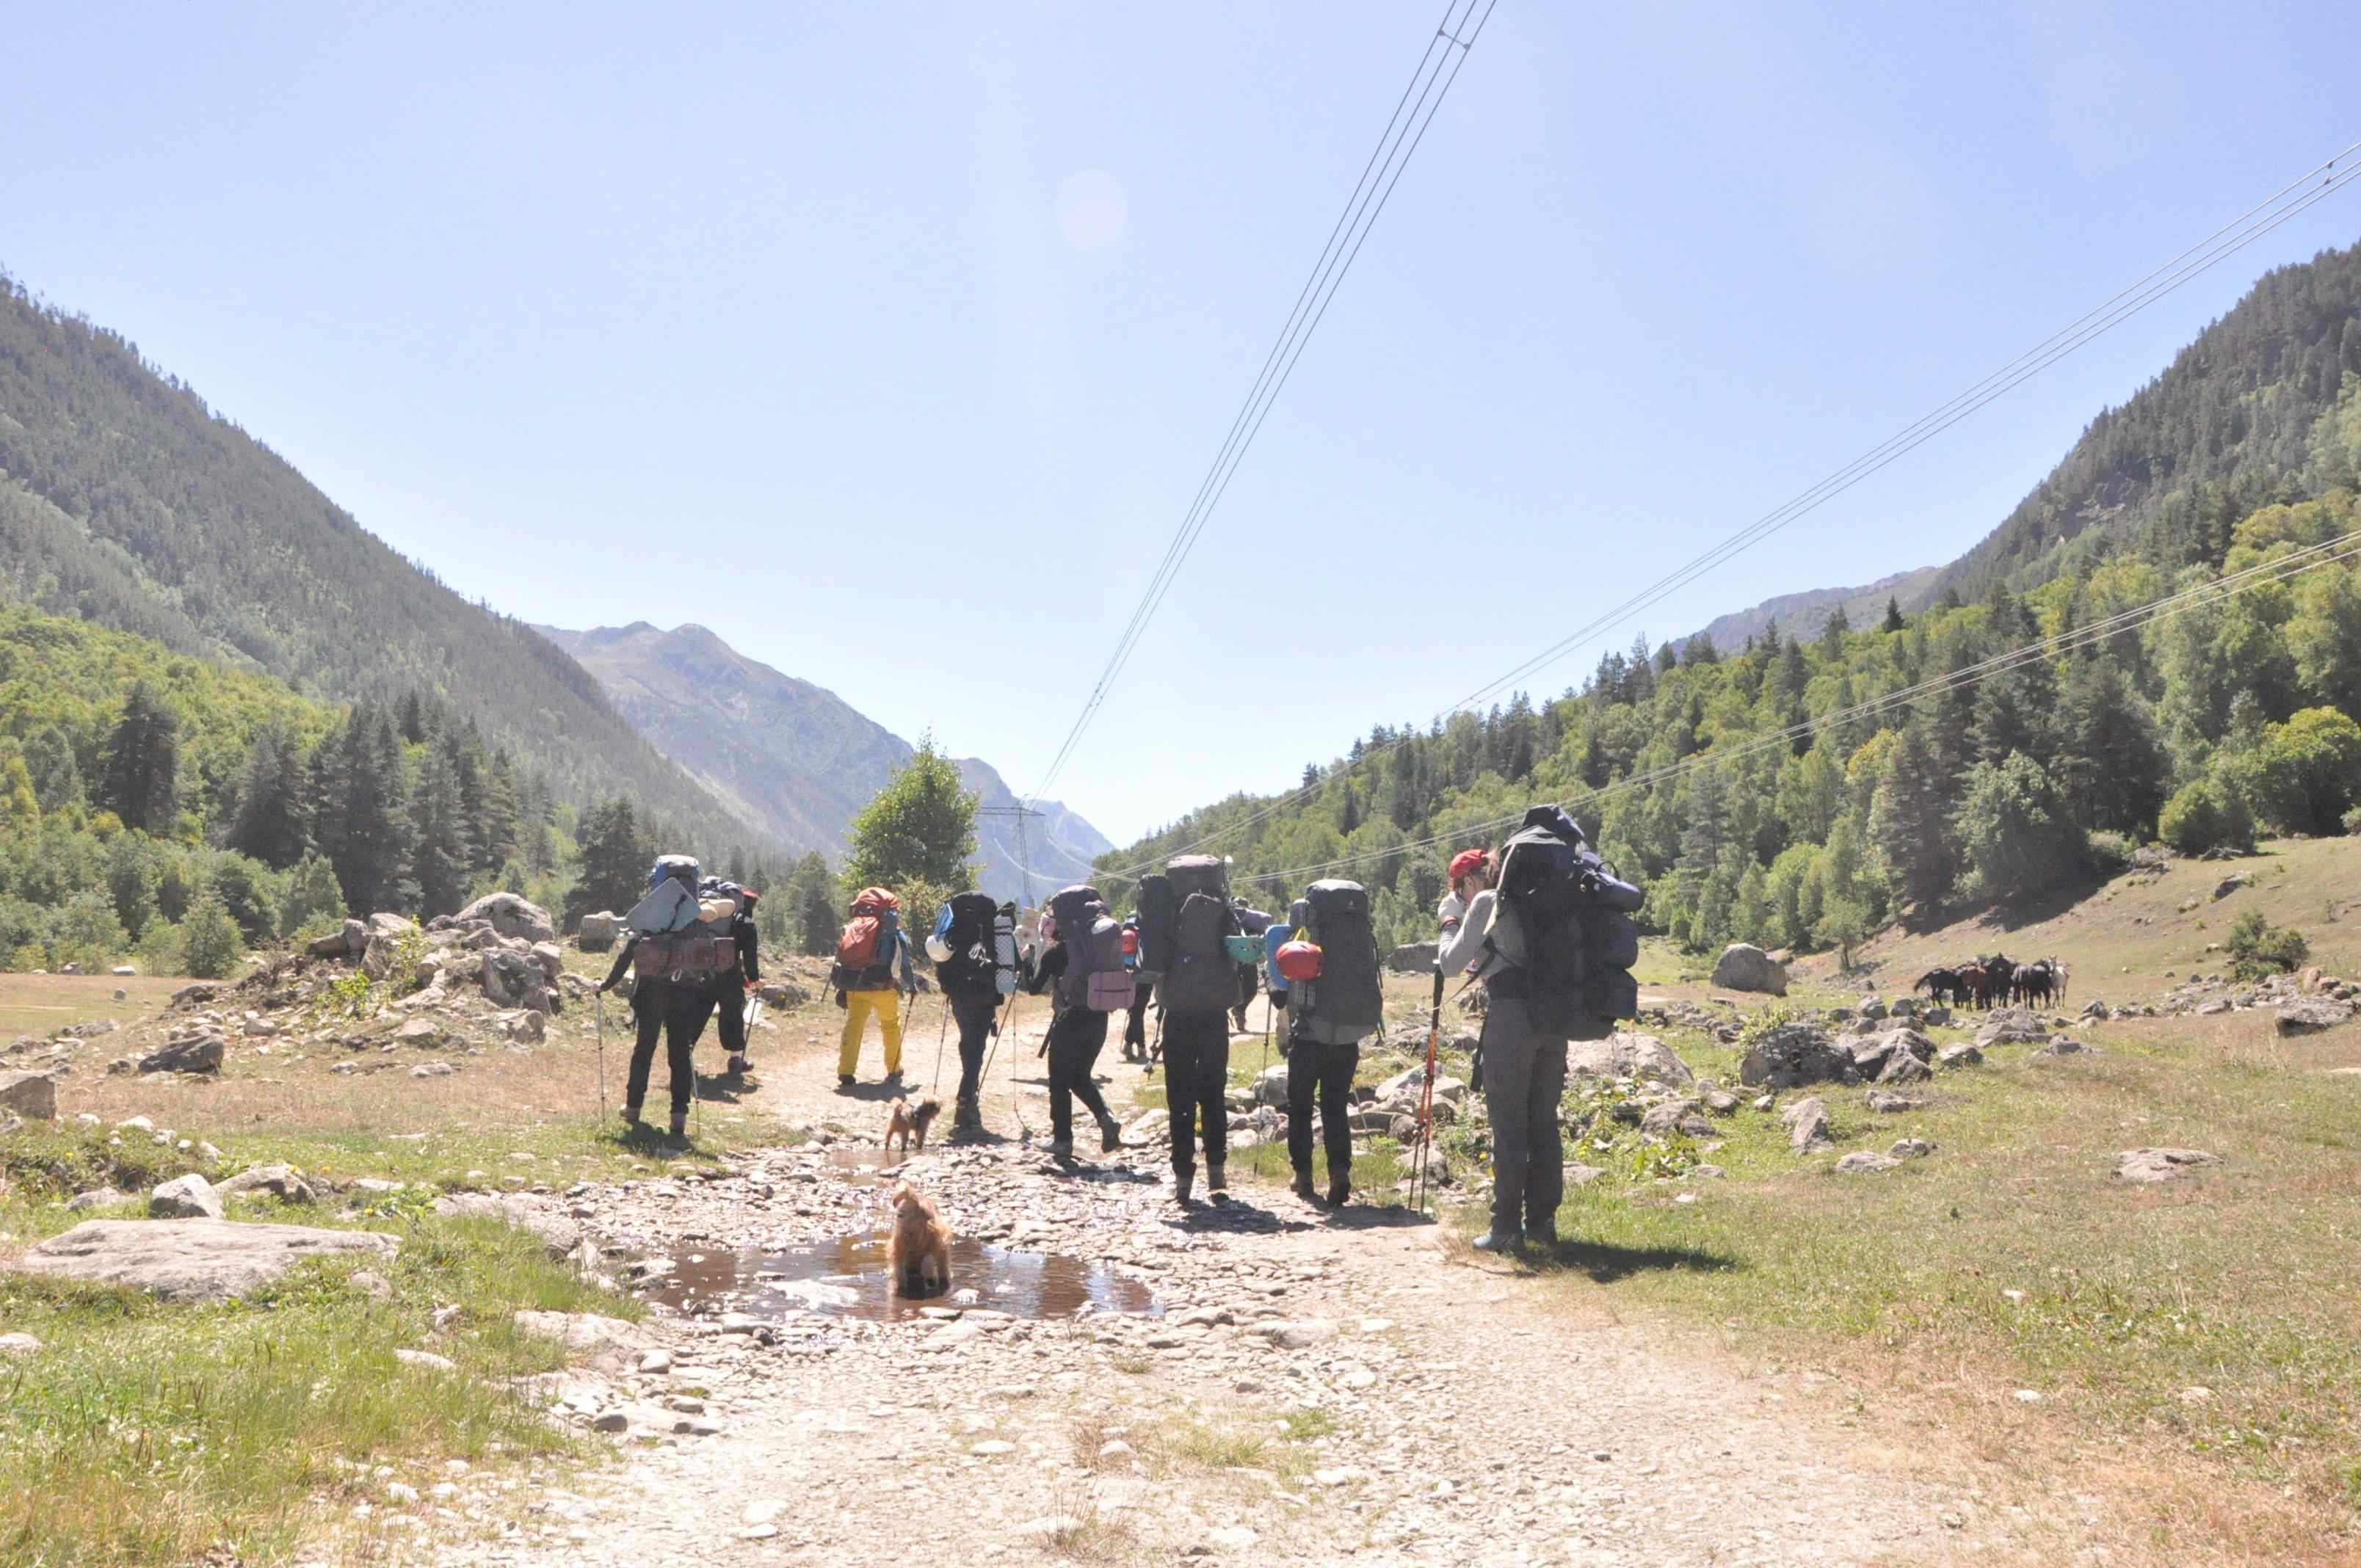
\includegraphics[width=\linewidth]{../pics/DSC_0412}
\end{frame}